\documentclass{article}

\usepackage{graphicx} % Required for the inclusion of images
\usepackage{natbib} % Required to change bibliography style to APA
\usepackage{amsmath} % Required for some math elements 
\usepackage[final]{pdfpages}
\usepackage[parfill]{parskip}
\usepackage{bm}

\usepackage[utf8]{inputenc}
\usepackage{mathpazo}
\usepackage[T1]{fontenc}
\usepackage{textcomp}
\usepackage{gensymb}
\usepackage{mathtools} 
\usepackage{algorithm}
\usepackage{algpseudocode}
\usepackage{booktabs}
\usepackage{caption}

\usepackage{amsmath,amsfonts,amssymb}

\usepackage{amssymb}
\usepackage{tikz}
\usetikzlibrary{arrows,shapes}

\tikzset{every picture/.style={remember picture}}

\setlength\parindent{0pt} % Removes all indentation from paragraphs

\renewcommand{\labelenumi}{\alph{enumi}.} % Make numbering in the enumerate environment by letter rather than number (e.g. section 6)

\newcommand{\grad}[1]{\nabla_{#1}}
\newcommand{\gradv}[1]{\nabla_{\bm{#1}}}
\newcommand{\thetab}{\bm{\theta}}
\newcommand{\phib}{\bm{\phi}}
\newcommand{\bP}{\bm{P}}
\newcommand{\bs}{\bm{s}}
\newcommand{\be}{\bm{e}}
\newcommand{\taub}{\bm{\tau}}
\newcommand{\sumparams}{\alpha(\bP,\thetab_i) + \beta(\bP, \thetab_i) + \gamma(\bP, \thetab_i) }

\long\def\/*#1*/{}

%----------------------------------------------------------------------------------------
%	DOCUMENT INFORMATION
%----------------------------------------------------------------------------------------

\title{Policy Search Approach for Power-efficient Arm Control}

\author{\textsc{Nick Walker}}

\date{CS394R Fall 2016} % Date for the report

\begin{document}
	
\maketitle % Insert the title, author and date

%----------------------------------------------------------------------------------------
%	SECTION 1
%----------------------------------------------------------------------------------------

\section{Motivation}

Motors consume substantial amounts of power, so it is important for a battery-powered mobile robotics systems to have an efficient motor usage policy. There are two components to an efficient motor policy. \textit{Utilization efficiency}, making movements only as necessary, and \textit{execution efficiency}, using joints to actuate movements as efficiently as possible. Speed is not the only component of execution efficiency. In some systems, there may be ways of using properties of the environment to transition between joint poses while  applying less torque. In an arm system for instance, a policy might use gravity to help it move towards the target configuration, even if it takes longer than a direct transition. While it is possible to plan power-optimal trajectories given a full model of the system, such models may be expensive or impossible to obtain. For these reasons, a learning approach, which can adapt to the idiosyncrasies of an individual platform, is of interest. In this project, I evaluate a policy search approach for optimizing a robotic arm's execution efficiency.


%----------------------------------------------------------------------------------------
%	SECTION 2
%----------------------------------------------------------------------------------------

\section{Introduction}

\subsection{Learning Platform}

I based the platform on the Teensy 3.2, an ARM Cortex-M4 development board. Compared to the popular AVR microcontrollers, ARM chips are substantially more powerful, and not much more expensive. Though both chips lack a floating point unit, ARM cores have an emulation advantage due to the their higher clock speed and native 32-bit operation capabilities. The Cortex line has seen substantial commercial use, so evaluating an embedded agent using the M4 provides useful insight into the constraints of real systems are.

\begin{center}
	\begin{tabular}{ l l l}
		& AtMega328p & Cortex-M4  \\ \midrule
		Instruction set & AVR & ARMv7-M\\
		Integer width & 8 bits & 32 bits\\
		SRAM & 2kb & 32kb\\
		Program memory & 32kb & 256kb\\
		Clock Speed & 16Mhz & 72Mhz\\ 
		FPU & No & No
		
	\end{tabular}
\end{center}

In order to provide a challenging task for the agent, I built a six degree of freedom arm. The arm's joints are MTR955 servos, each capable of 170$\degree$ of rotation, though some joints have less range of motion to physical constraints.

\begin{center}
	\begin{tabular}{ l l l}
		Joint & Rotation range ($\deg$)  \\ \midrule
		0 & 160 \\
		1 & 120 \\
		2 & 50 \\
		3 & 50 \\
		4 & 50\\ 
		5 & 30
		
	\end{tabular}
\end{center}

\begin{figure}
	\centering
	%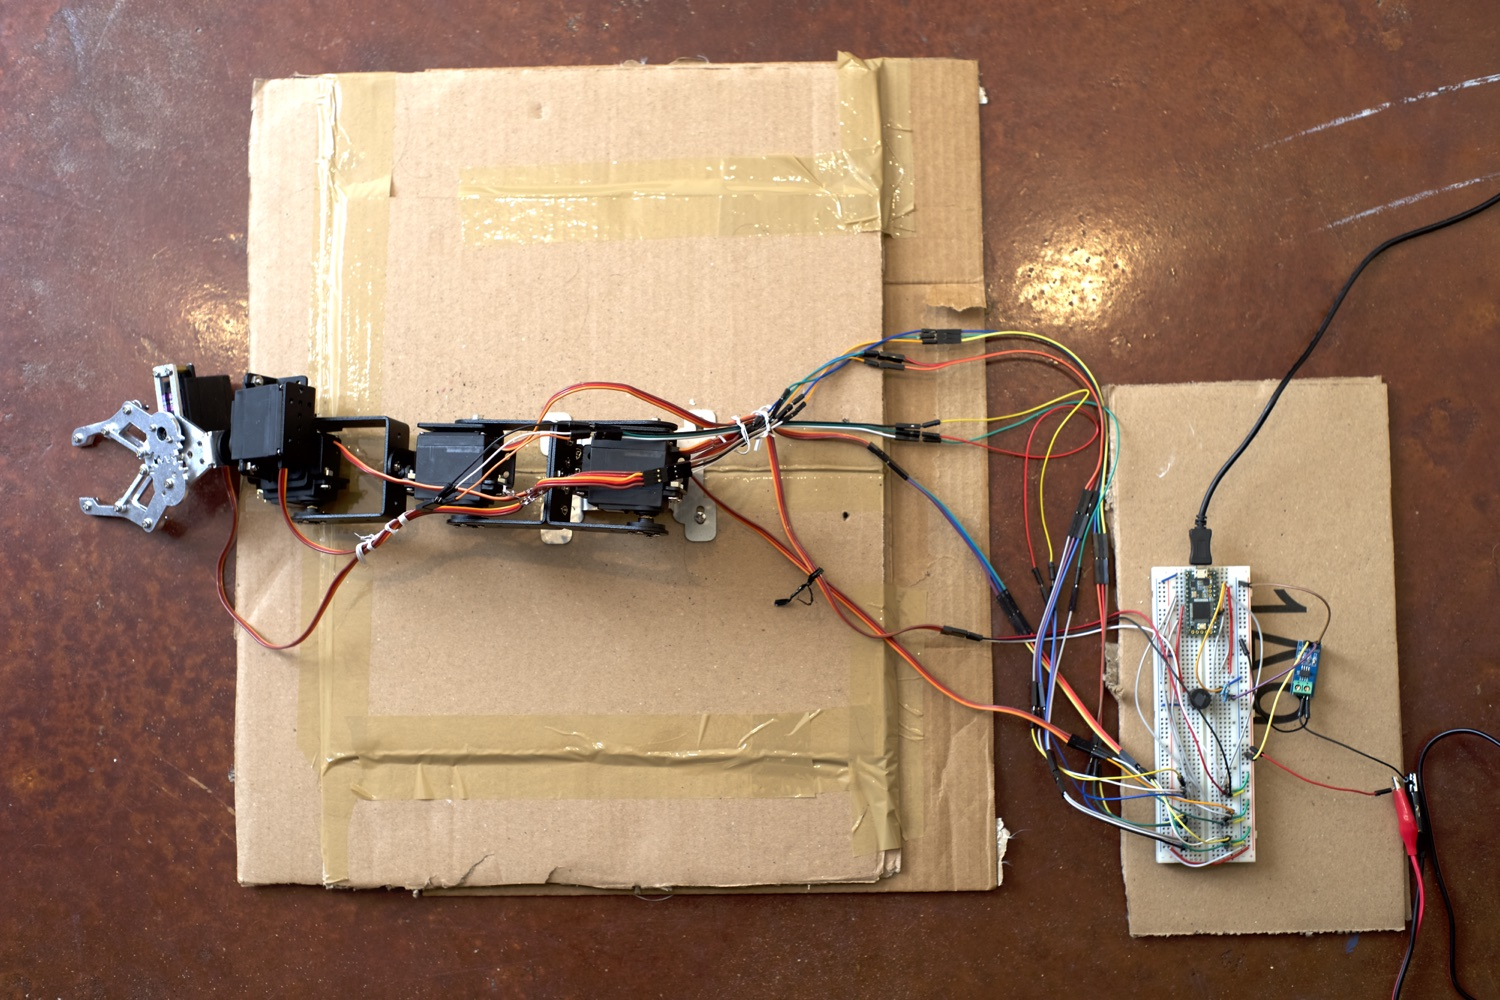
\includegraphics[width=10cm]{../photos/eagle_small.jpg}
	%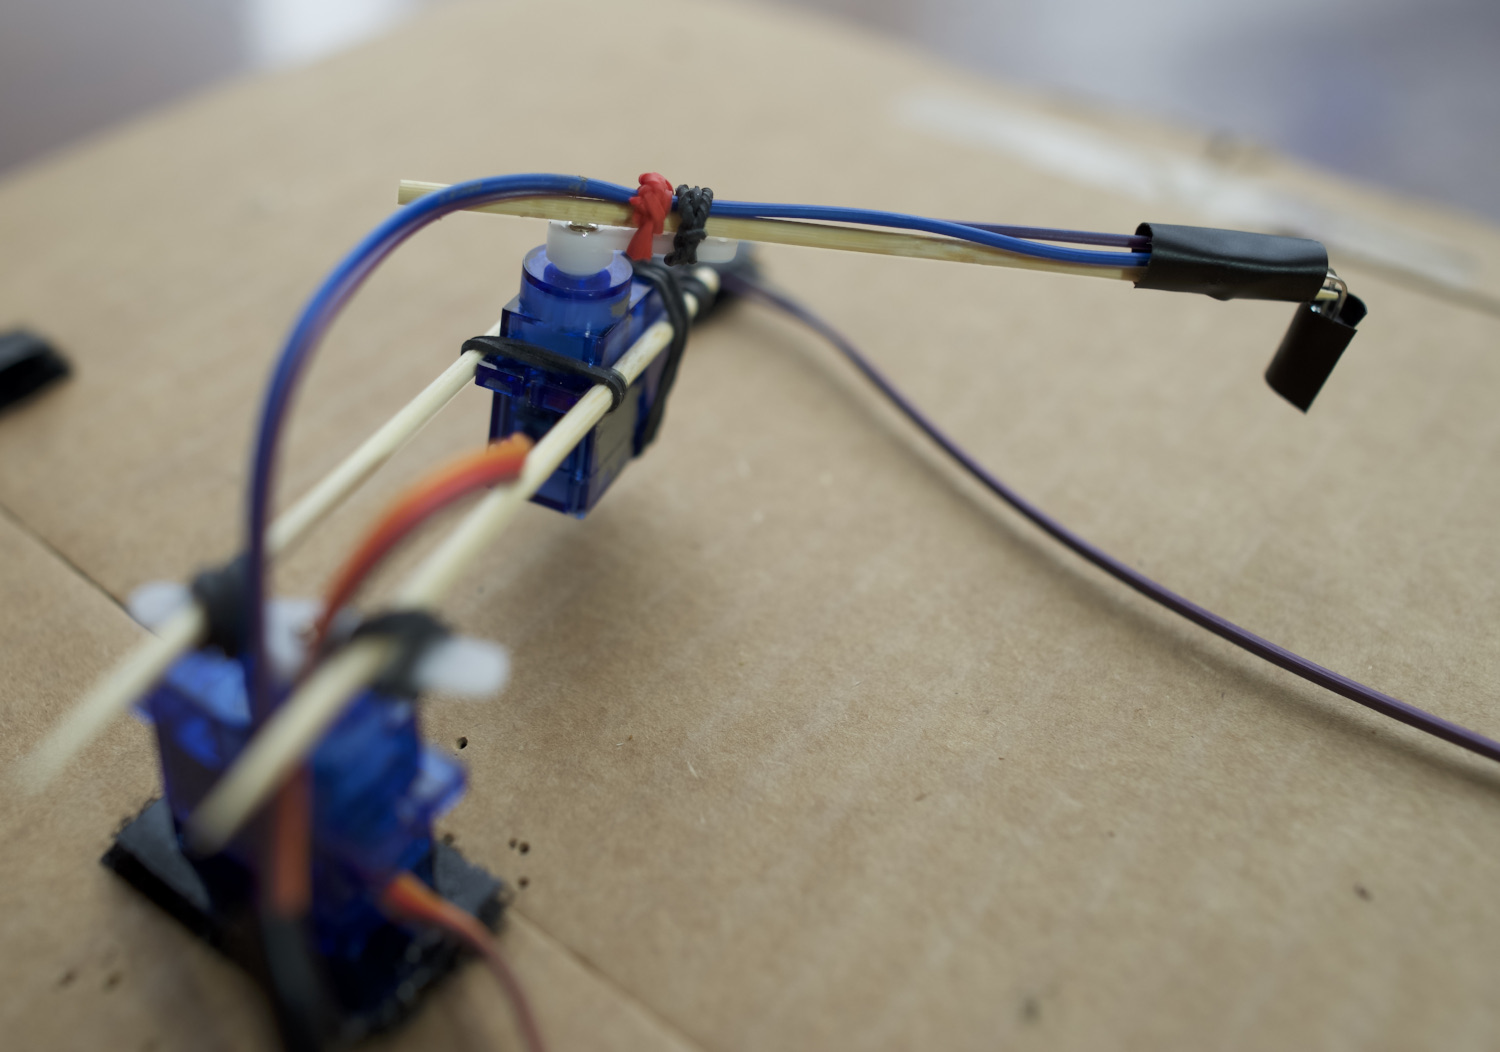
\includegraphics[width=10cm]{../photos/arm_detail_small.jpg}
	\caption{Top: The learning platform. Five joints control the articulation of the arm, while the sixth opens and closes the grasper.}
	\label{fig:platform}
\end{figure}


\subsection{Problem}

The arm is given a command $\bP$ consisting of initial and ending poses (joint angles).

\begin{equation}
	\bP = [\bm{i}, \be]\\
\end{equation}

The agent must move all of its joints into the end pose, using as little energy as possible. The current usage of the system is monitored continuously, and the agent is given the negative power usage of its trajectory as its reward.


\subsection{Approach}

The servo controller library used for this project allows joint angles to be specified with single degree precision, making the space of possible joint configurations and actions essentially continuous. Value function methods face significant challenges in such a domain, and are infeasible given the platform constraints of this problem, so a policy search method must be used.

The book presents one possible policy parameterization for a continuous state-action problem, a normal distribution over a scalar real-valued action with parameterized mean and variance. This form of policy doesn't encode the useful knowledge that the trajectory must always end at the target configuration.

I instead chose to provide a custom policy. For initial arm pose $\bm{i}$ and end arm pose $\bm{e}$, a joint $j_i$'s angle at time $t$ is given by a cubic polynomial interpolation from $s_i$ to $e_i$. The polynomial's coefficients must be positive, and are modeled as the exponentiation of a linear function of the start and end arm pose and per-joint weights. To ensure safe operation, individual joint trajectories are executed slower or faster such that, for $t$ in $[0,1]$, they have a maximum angular velocity of exactly $10\degree$/s. An additional per-joint parameter, $\delta$ allows the curve velocity to be scaled down further, preserving the ability to represent policies that move joints slowly.
\begin{gather}
	\bm{T} = [\thetab_0, \thetab_1, \thetab_2, \thetab_3, \thetab_4, \thetab_5]\\
	\thetab_i = [\taub_\alpha, \taub_\beta, \taub_\gamma, \taub_\delta] \\
	j_i(t, \bP | \bm{T}) = \be_i\bigg (\frac{\alpha(\bP,\thetab_i) t^3 + \beta(\bP, \thetab_i) t^2 + \gamma(\bP, \thetab_i) t}{\sumparams}\bigg) + \bm{i}_i\\
	\alpha(\bP,\thetab_i) = \exp(\taub_\alpha^\top \phib_s)\\
	\beta(\bP,\thetab_i) = \exp(\taub_\beta^\top \phib_s)\\
	\gamma(\bP,\thetab_i) = \exp(\taub_\gamma^\top \phib_s)\\	
	\delta(\bP,\thetab_i) = \frac{1}{\exp(\taub_\delta^\top \phib_s) + 1}
\end{gather}

This policy, including the safety transformation, is differentiable, but the gradient calculation is complex and challenging to implement given the memory constraints of the platform. In the interest of evaluating the cubic polynomial interpolation policy format quickly, I used the finite difference algorithm from \cite{stone2006} and directly sampled the gradient instead of computing it. Because this approach requires a number of rollouts proportional to the size of $\thetab$,  I restricted my evaluation of the approach to a fixed $\bm{s}$ and $\bm{e}$, reducing the problem to direct optimization of $\alpha$, $\beta$, $\gamma$, and $\delta$ for each joint.
	

%----------------------------------------------------------------------------------------
%	SECTION 3
%----------------------------------------------------------------------------------------

\section{Experimental Setup}

The agent is allowed to execute 100 iterations of the algorithm. Each iteration, it performs 24 rollouts to sample the gradient, using parameters perturbed by one of $[-0.1, 0.0, 0.1]$. A step size of 0.05 is used to update the parameters after the gradient is sampled, then an evaluation of the new weights is recorded.

%----------------------------------------------------------------------------------------
%	SECTION 4
%----------------------------------------------------------------------------------------


\section{Results}


	\begin{figure}[h]
		\begin{center}
			%\includegraphics[width=\textwidth]{figure_0.pdf}
			\caption{Results of an evaluation}
		\end{center}
	\end{figure}
	
\subsection{Discussion}

The agent learns and generalizes a fairly good policy within its first fifty steps. The evaluation period demonstrates that the learned policy performs well from arbitrary start positions. 

Even though it points the LED at the photocell consistently, the agent does not learn the LED reward dynamics. As can be seen in the video\footnote{https://youtu.be/SCv1AomFDG0}, it opts to leave the light on at all times. This is not unexpected, since it lacks features that describe the interaction of the joint position with the value of actions that turn the LED on. The weight associated with the LED activation action-feature is forced to represent the value of LED actions from any state. Averaged across the entire state space, turning the light on has a higher value than turning it off, so it always leaves it on. Efficient LED activation is not as important as joint movement, so it seems reasonable to prioritize detailed state-space representation over features that would better capture the use of the light.



%----------------------------------------------------------------------------------------
%	SECTION 5
%----------------------------------------------------------------------------------------

\section{Conclusions}



\clearpage

\/*
\section{Appendix A: Images}

	\begin{figure}[!htb]
		\centering
		\includegraphics[width=10cm]{../photos/.jpg}
		\label{fig:}
	\end{figure}
	
	\begin{figure}[!htb]
		\centering
		\includegraphics[width=10cm]{../photos/.jpg}
		\caption{}
		\label{fig:}
	\end{figure}
	
	\begin{figure}[!htb]
		\centering
		\includegraphics[width=10cm]{../photos/.jpg}
		\caption{}
		\label{fig:}
	\end{figure}
*/

\section{Appendix B: Bill of Materials}


\begin{center}
	\begin{tabular}{ l c c  p{5cm} }
		\toprule
		Component & Quantity & Unit Price (\$) & Note \\ \midrule
		Teensy 3.2 & 1 & 18.00 &  \\ 
		MTR955R servo & 6 & 4.00 & Any standard servo.\\ 
		Arm kit & 1 & 30.00 & \\
		ASC112 current sensor & 1 & 4.00 & Or similar\\
		5v 5.0A power supply & 1 & 16.00 & If variable supply unavailable. \\ 
		Breadboard & 1 & 4.00 & \\
		Assorted jumpers & & 3.00 & \\
		Adhesives, project surface & & 4.00 & \\
		\bottomrule
		
	\end{tabular}
\end{center}

	
\end{document}
